%!TEX root = ../report.tex

\begin{document}
    \chapter{Introduction}

%-------------------------------------------------------------------------------
%	Motivation
%-------------------------------------------------------------------------------
    \section{Motivation}
    
        Every day, people are exposed to some kind of accident, and the worst kind of accidents are those that put their lives at risk.
        Fortunately, for those kinds of accidents, we have rescue services like firefighters.
        Nevertheless, firefighters are humans and put their lives at risk trying to save other people.
        According to the Deutscher Feuerwehrverband (German Firefighters Association), the number of firefighters missions in Germany in 2017 
        reached more than 3 million, and the number of deaths in fires in 2016 was approximately 350 \cite{DeutscherFeuerweherverband_online}.
        \par
        What if the firefighters are supported by rescue robots?
        With the use of rescue robots that explore the accident areas, we can help firefighters do their job more safely.
        Rescue robots can explore buildings to find entrances, exits, and other key areas that help firefighters rescue people faster and more efficiently.
        However, robots cannot find their exact position inside a building with a single GPS because this kind of technology is unreliable under certain conditions 
        (e.g., inside buildings).
        \par
        In this work, we try to enable rescue robots to explore buildings using LiDAR systems and 3D models of the buildings.
        With the use of LiDAR systems, we can obtain representations of the current state of buildings at risk without endangering any lives. 
        These kinds of representations are known as point clouds.
        \par
        With the use of CityGML models \cite{Groger_2012_OGC}, we have access to the 3D representation of many buildings in Germany.
        CityGML models can be presented in different Levels of Detail (LOD), from the coarsest level LOD0 to the most refined level LOD4.
        In LOD0, buildings can be represented by a simple footprint. While in LOD4, buildings contain information about windows, doors, stairs, and other internal structures.
        Unfortunately, not all models are LOD4. Even if they were, the information might be outdated. For example, it may be that due to some collapse, some door or window is blocked.
        \par
        Using modern registration techniques, one can find a match between the point cloud given by the LiDAR system and the 3D model of the building.
        The registration result can then be used to find the robot’s exact position with respect to the building.
        The registration result can also help locate relevant parts of the building, like windows, doors, stairs, or corridors.
        This information can be presented to the firefighters in a way that enables them to design a rescue plan, with the only objective of 
        supporting firefighters in their mission to rescue lives and safeguard theirs.

%-------------------------------------------------------------------------------
%	Challenges and Difficulties
%-------------------------------------------------------------------------------
    \section{Challenges and Difficulties}
    
        Most of the registration algorithms are focused on working with two point clouds.
        Just a few registration algorithms address the registration of 3D models with point clouds.
        Moreover, between those registration algorithms, only a couple are created to work with CityGML models, as described in \autoref{chap:State of the Art}.
        \par      
        The registration process is usually done by hand because it is a simple task for humans since we all learn to match patterns when we are just children. 
        Automatic registration is complicated because it is difficult for a computer to find features and match them between two different types of 3D data.
        \par
        An additional challenge is the data itself. The available point clouds are partial, they do not represent the whole 3D model, 
        and they usually just capture part of the walls of the buildings and the surface outside the buildings. 
        In contrast, the 3D models do not have information about the surface outside the buildings. 
        The only information available in both the 3D models and the point cloud is some of the walls of the buildings.
        \par
        

%-------------------------------------------------------------------------------
%	Problem Statement
%-------------------------------------------------------------------------------
    \section{Problem Statement}
        This work intends to implement an automated registration method for a point cloud with a CityGML model.
        This automated registration method will then be used as part of the A-DRZ (Aufbau des Deutschen Rettungsrobotik-Zentrums) \cite{A-DRZ_online} project of the Fraunhofer IAIS.
        \autoref{fig:adrz} shows the system architecture of the A-DRZ project. 
        The final objective of the automated registration in the A-DRZ project is to look inside the CityGML models
        to find the location and state of relevant parts of the buildings (e.g., doors, windows, stairs, and corridors) that can be used for rescue tasks.
        
        \begin{figure}[htp]
            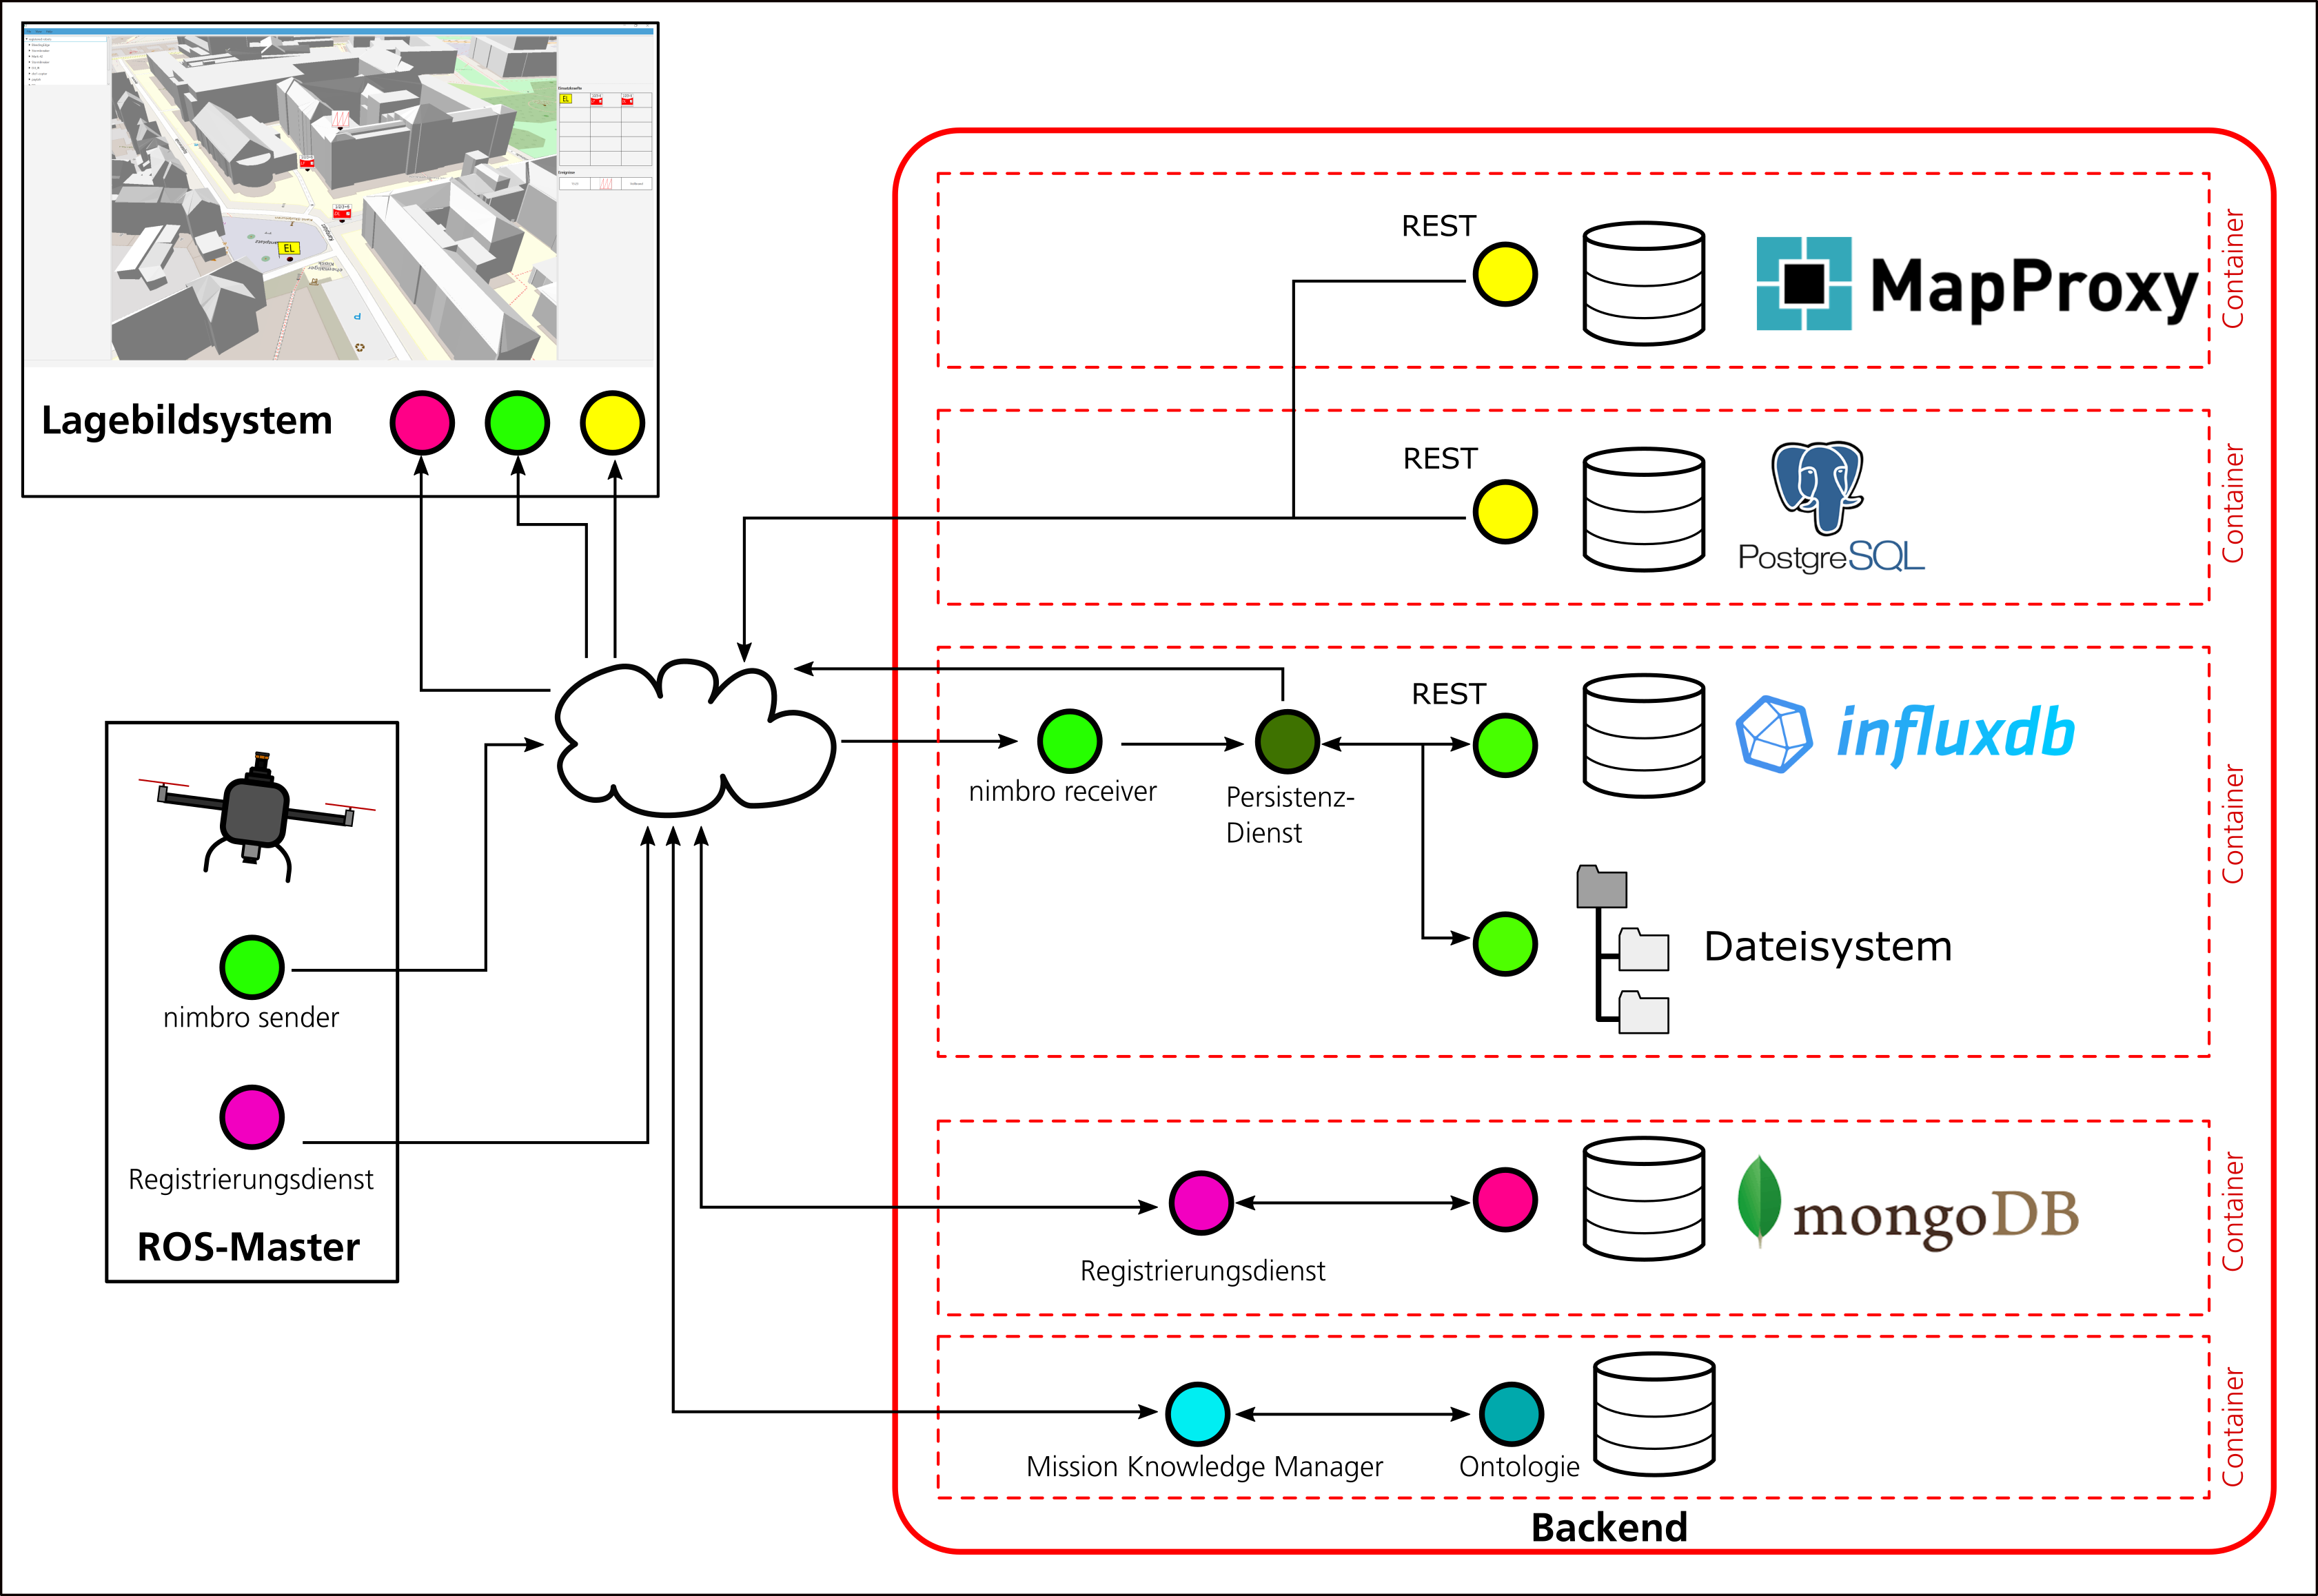
\includegraphics[width=\textwidth]{images/Systemaufbau.png}
            \caption{A-DRZ architecture system (Image provided by the Fraunhofer IAIS).}
            \label{fig:adrz}
        \end{figure}

        The current automated approaches are mainly focused on point-to-point registration.
        Therefore, the exploration of point-to-model automated registration methods is necessary to implement a solution that aims to work in real-time.
        Moreover, there is no automated process implemented in the A-DRZ project yet. 
        However, as an assistance system, the A-DRZ project should avoid human interaction for performing the registration.

        \autoref{fig:system_diagram} shows the general workflow of the required method.
        The method’s input is a point cloud and the corresponding CityGML model of a building  
        (the process to obtain this input is outside of the scope of this work).
        The provided input is preprocessed and used for the registration algorithm.
        The output of the registration algorithm is a transformation that maps the point cloud to the CityGML model.
        Finally, the output transformation and the input data are used to visualize the point cloud on the CityGML model.

        \begin{figure}[htp]
            \centering
            \includesvg[width=\columnwidth,inkscapelatex=false]{images/diagramR}
            % 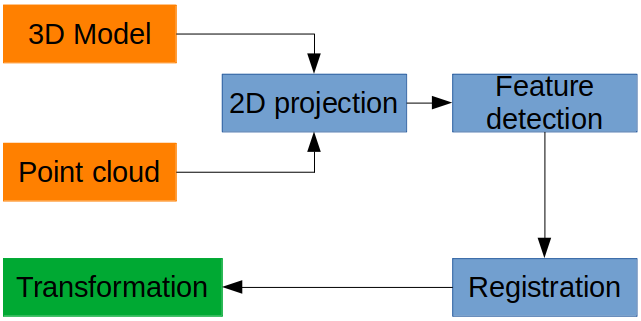
\includegraphics[scale=0.5]{images/RegistrationProcess}
            \caption{System diagram.}
            \label{fig:system_diagram}
        \end{figure}

        First, the resulting algorithm will be tested manually. 
        If the results are the expected ones, the resulting algorithm will be integrated into a visualization software from the Fraunhofer IAIS. 
        At the moment, this visualization software is, in general, a 3D rendering of CityGML models limited to a particular geographical area.


\end{document}
